Chương này trình bày các thí nghiệm nhằm đánh giá hiệu quả hoạt động của giải pháp định tuyến sử dụng thuật toán Gradient triển khai trên các nút sử dụng vi xử lý nRF54L15 Nordic: 1) Đánh giá độ chính xác việc thiết lập định tuyến trên các nút; 2) Đánh giá khả năng truyền nhận tin trong mạng khi sử dụng định tuyến dựa trên gradient. Cụ thể khóa luận đã thực hiện 3 thí nghiệm như sau:
\section{Thí nghiệm 1: Mạng cấu trúc tĩnh}  
\label{sec:static_network}

Thí nghiệm đầu tiên được thiết kế để đánh giá hiệu suất của thuật toán định tuyến Gradient trên các mạng có cấu trúc cố định, không thay đổi trong suốt quá trình thí nghiệm. Mục tiêu chính là kiểm chứng khả năng thiết lập gradient, độ tin cậy trong việc chuyển tiếp dữ liệu, và tỷ lệ truyền tin thành công.

\subsection{Thiết lập thí nghiệm}

\subsubsection{Phần cứng sử dụng}

Thí nghiệm được thực hiện trên hệ thống gồm nhiều mạch custom như trong hình \ref{fig:nRF54L15EZDK} với vi điều khiển chính là nRF54L15 DK của Nordic Semiconductor. Phần anten phát BLE của mạch nằm ở vị trí được khoanh đỏ, do đó mạch sẽ phát và nhận tín hiệu tốt hơn theo hướng này. Mỗi mạch nRF54L15-EZDK đóng vai trò một node trong mạng BLE Mesh, được nạp chung 1 firmware với Gradient Server Model đã phát triển. Các node được đặt tại các vị trí cố định trong không gian thí nghiệm. Khoảng cách giữa cách node là khoảng 30 cm. Một node được chỉ định làm sink node với gradient cố định bằng 0, đóng vai trò điểm thu thập dữ liệu trung tâm.

\begin{figure}[h!]
    \centering
    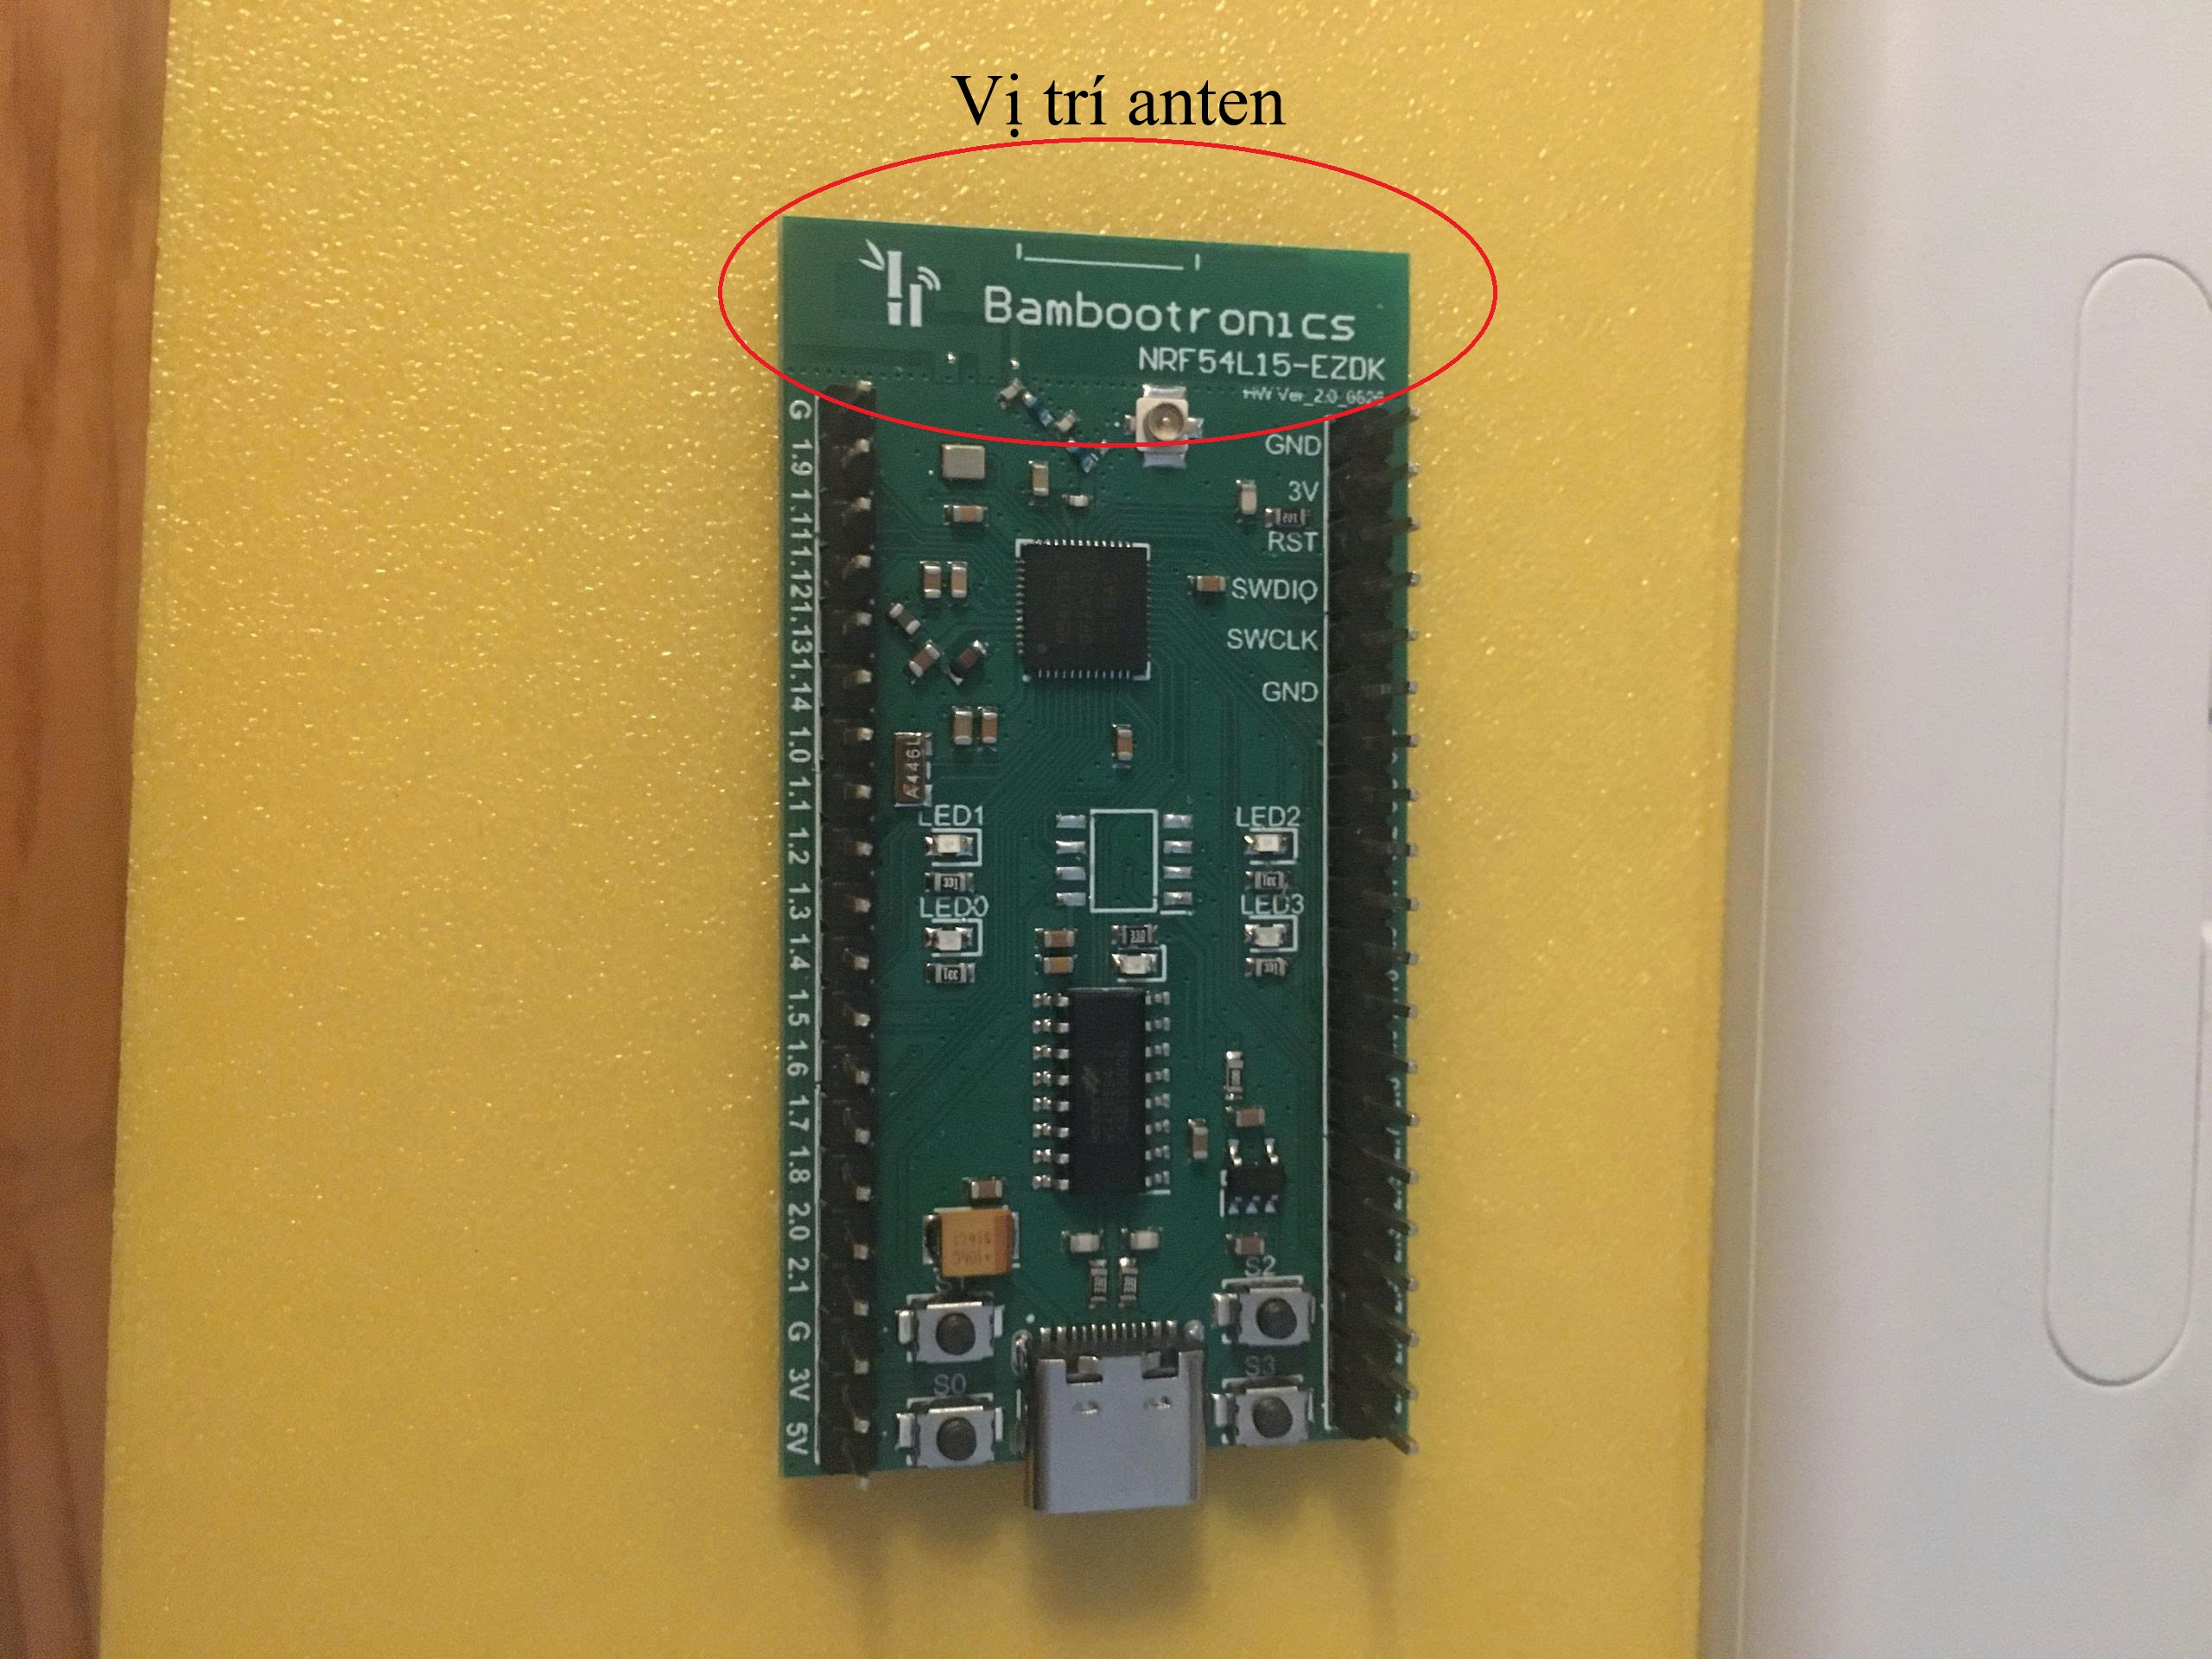
\includegraphics[width=0.65\textwidth]{chapter2/image/nRF54L15EZDK.jpg}
    \caption{Mạch nRF54L15-EZDK được sử dụng trong thí nghiệm}
    \label{fig:nRF54L15EZDK}
\end{figure}

\subsubsection{Cấu hình các node mạng}

Gradient Server Model được tích hợp vào BLE Mesh stack với các tham số cấu hình như sau:
\begin{itemize}
    \item Chu kỳ broadcast GRADIENT\_STATUS: 5 giây
    \item Timeout cho Forwarding Table entry: 30 giây
    \item Kích thước tối đa Forwarding Table: 3 entries
    \item Công suất phát: -12 dBm
\end{itemize} 
Việc đặt công suất phát ở mức -12 dBm nhằm có thể dễ dàng thực hiện thí nghiệm trong không gian hẹp thay vì phải lắp đặt ở không gian rộng lớn. Mỗi sensor node được cấu hình gửi một gói tin DATA khi Button 0 được nhấn, chứa payload gồm giá trị counter tăng dần (2 bytes). 

\subsubsection{Tiêu chí đánh giá}

Hiệu suất của giải pháp được đánh giá dựa trên các tiêu chí: 
\begin{itemize}
    \item Tính chính xác trong xây dựng và cập nhật bảng định tuyến trên node.
    \item Hiệu suất dựa trên tỷ lệ phần trăm gói tin DATA được gửi từ sensor node và nhận thành công tại sink node
\end{itemize}

\subsubsection{Phần mềm debug}

Sử dụng Serial Terminal trong bộ công cụ nRF Connect for Desktop để giám sát các gói tin BLE Mesh được gửi và nhận trong mạng và bảng định tuyến của các node mạng. 

\subsection{Topology mạng dạng cây}
Topology dạng cây là cấu trúc phân cấp trong đó sink node nằm ở gốc cây, và các node khác được sắp xếp thành các tầng. Thí nghiệm sử dụng topology cây với 10 node được bố trí như Hình \ref{fig:tree_topology}, trong đó sink node (gradient = 0) nằm ở vị trí trung tâm trên cùng, các node tầng 1 có gradient = 1 kết nối trực tiếp với sink, và các node tầng 2 có gradient = 2 kết nối thông qua các node tầng 1, tương tự với các node tầng tiếp theo.

\begin{figure}[h!]
    \centering
    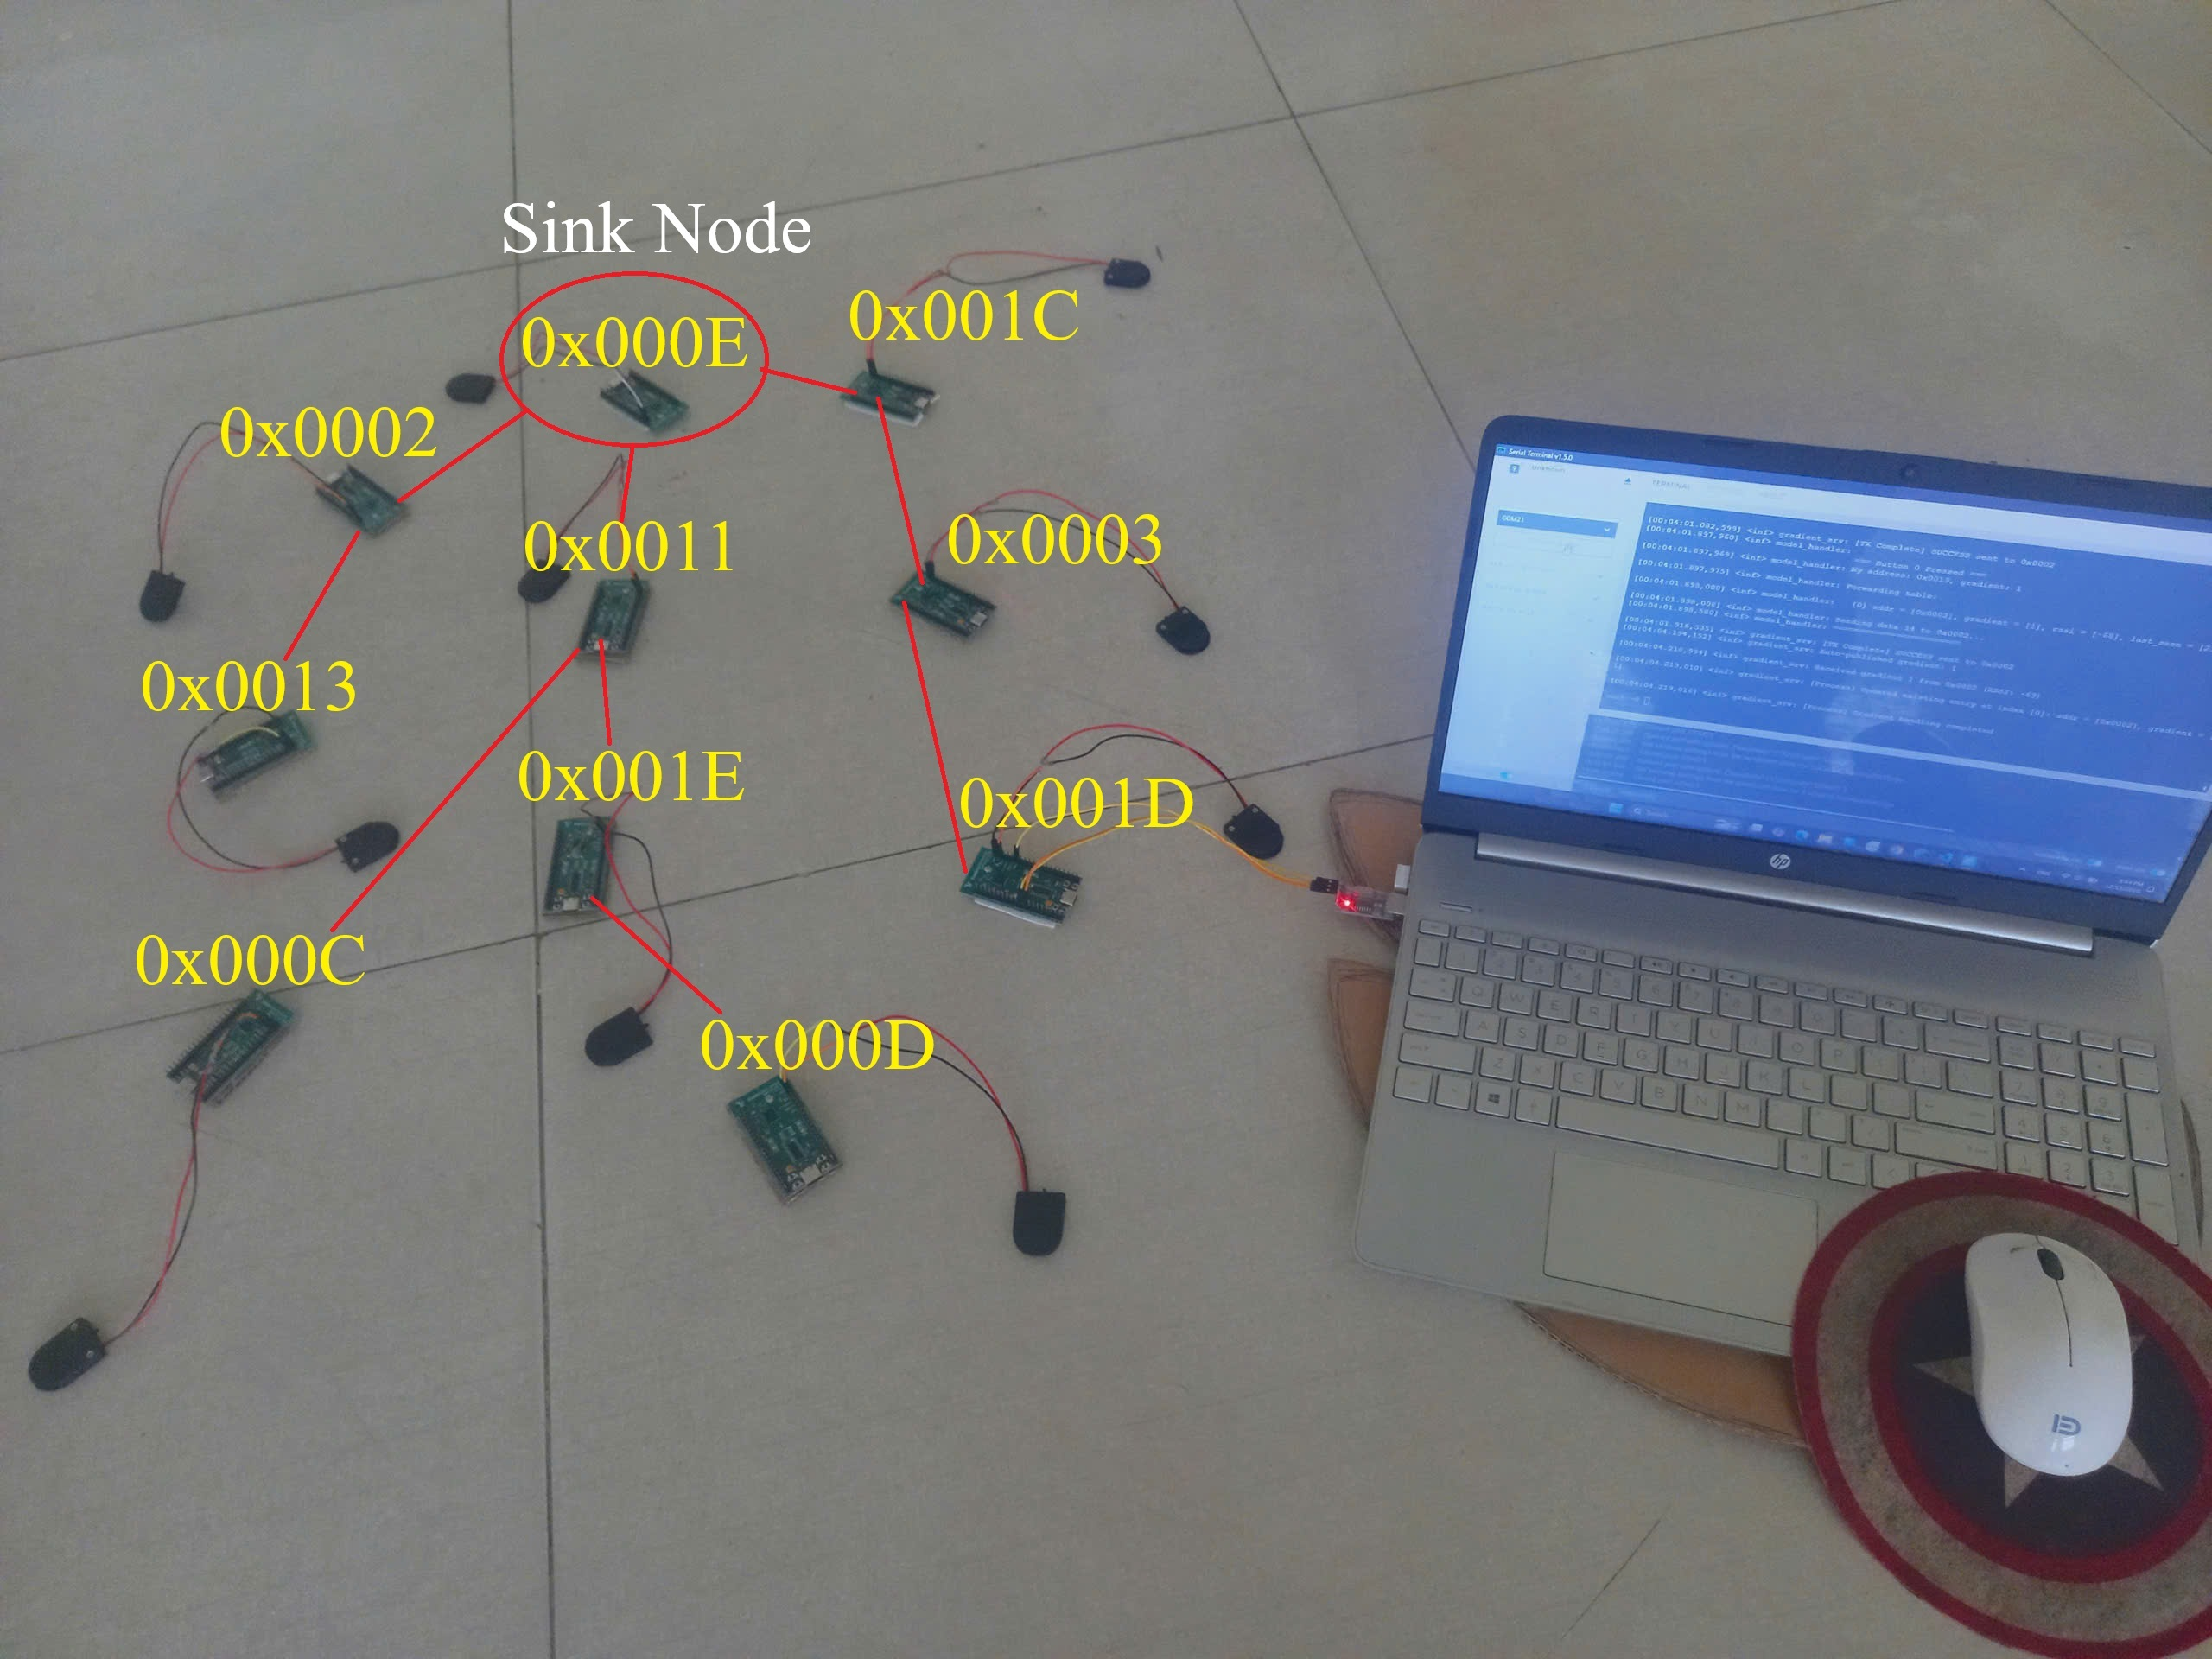
\includegraphics[width=0.50\textwidth]{chapter2/image/demo.jpg}
    \caption{Topology mạng thí nghiệm dạng cây}
    \label{fig:tree_topology}
\end{figure}

\clearpage

Tiến hành check log trên từng node trong mạng để kiểm tra bảng định tuyến sau khi quá trình thiết lập gradient hoàn tất. Kết quả hiển thị trong Hình\ref{fig:tree_topology_routing_table}.

\begin{figure}[h!]
    \centering
    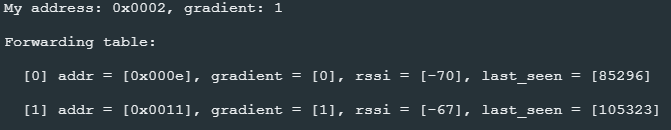
\includegraphics[width=0.75\textwidth]{chapter2/image/0x0002.png}
    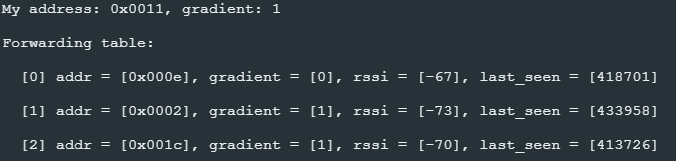
\includegraphics[width=0.75\textwidth]{chapter2/image/0x011.png}
    \includegraphics[width=0.75\textwidth]{chapter2/image/0x01C.png}
    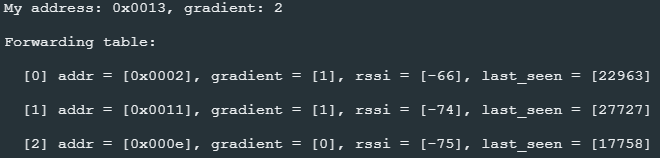
\includegraphics[width=0.75\textwidth]{chapter2/image/0x013.png}
    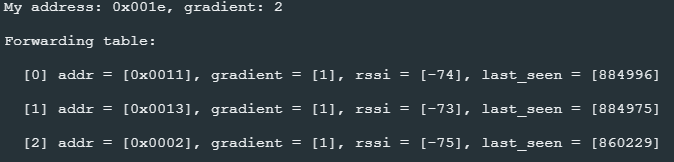
\includegraphics[width=0.75\textwidth]{chapter2/image/0x001E.png}
    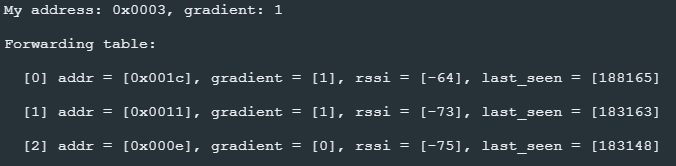
\includegraphics[width=0.75\textwidth]{chapter2/image/0x0003.png}
    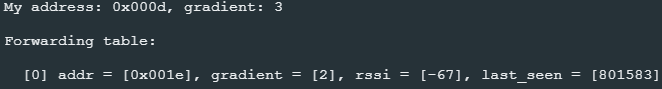
\includegraphics[width=0.75\textwidth]{chapter2/image/0x000D.png}
    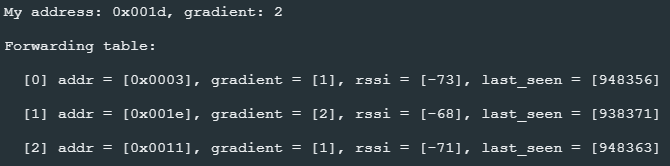
\includegraphics[width=0.75\textwidth]{chapter2/image/0x001D.png}
    \caption{Bảng định tuyến tại node các node trong mạng}
    \label{fig:tree_topology_routing_table}
\end{figure}

\clearpage

\subsubsection{Giải thích kết quả}
Khi mạng được khởi tạo, Sink node publish GRADIENT\_STATUS với gradient = 0. Các node có địa chỉ 0x0002, 0x0011 và 0x001C nhận được và cập nhật gradient = 1, sau đó Publish lại GRADIENT\_STATUS với gradient = 1. Node 0x0013 nhận được gradient = 1 từ node 0x0002 và 0x0011 và cập nhật gradient = 2, tương tự node 0x001E, 0x000C, và 0x0003 cũng nhận được gradient = 1 và cập nhật Gradient = 2. Cuối cùng các node 0x000D và 0x001D nhận được Gradient = 2 từ lần lượt các node 0x001E và 0x0003 và cập nhật gradient = 3. 

\subsubsection{Kết quả thí nghiệm}

Các node trong mạng đã thiết lập gradient thành công theo đúng cấu trúc cây. Đồng thời, vị trí các hàng xóng trong bảng định tuyến cũng được sắp xếp đúng theo thứ tự tăng dần của gradient và giảm dần của RSSI, đảm bảo rằng các node sẽ ưu tiên chọn next-hop có gradient thấp nhất và liên kết tốt nhất để chuyển tiếp gói tin DATA.

Kết quả sau khi thực hiện 100 lần truyền gói tin DATA từ các sensor node đến sink node cho thấy tỷ lệ truyền thành công là 100\%.

\subsection{Topology mạng dạng lưới}

Topology thí nghiệm được thiết lập như trên hình \ref{fig:grid_topology}
\begin{figure}[h!]
    \centering
    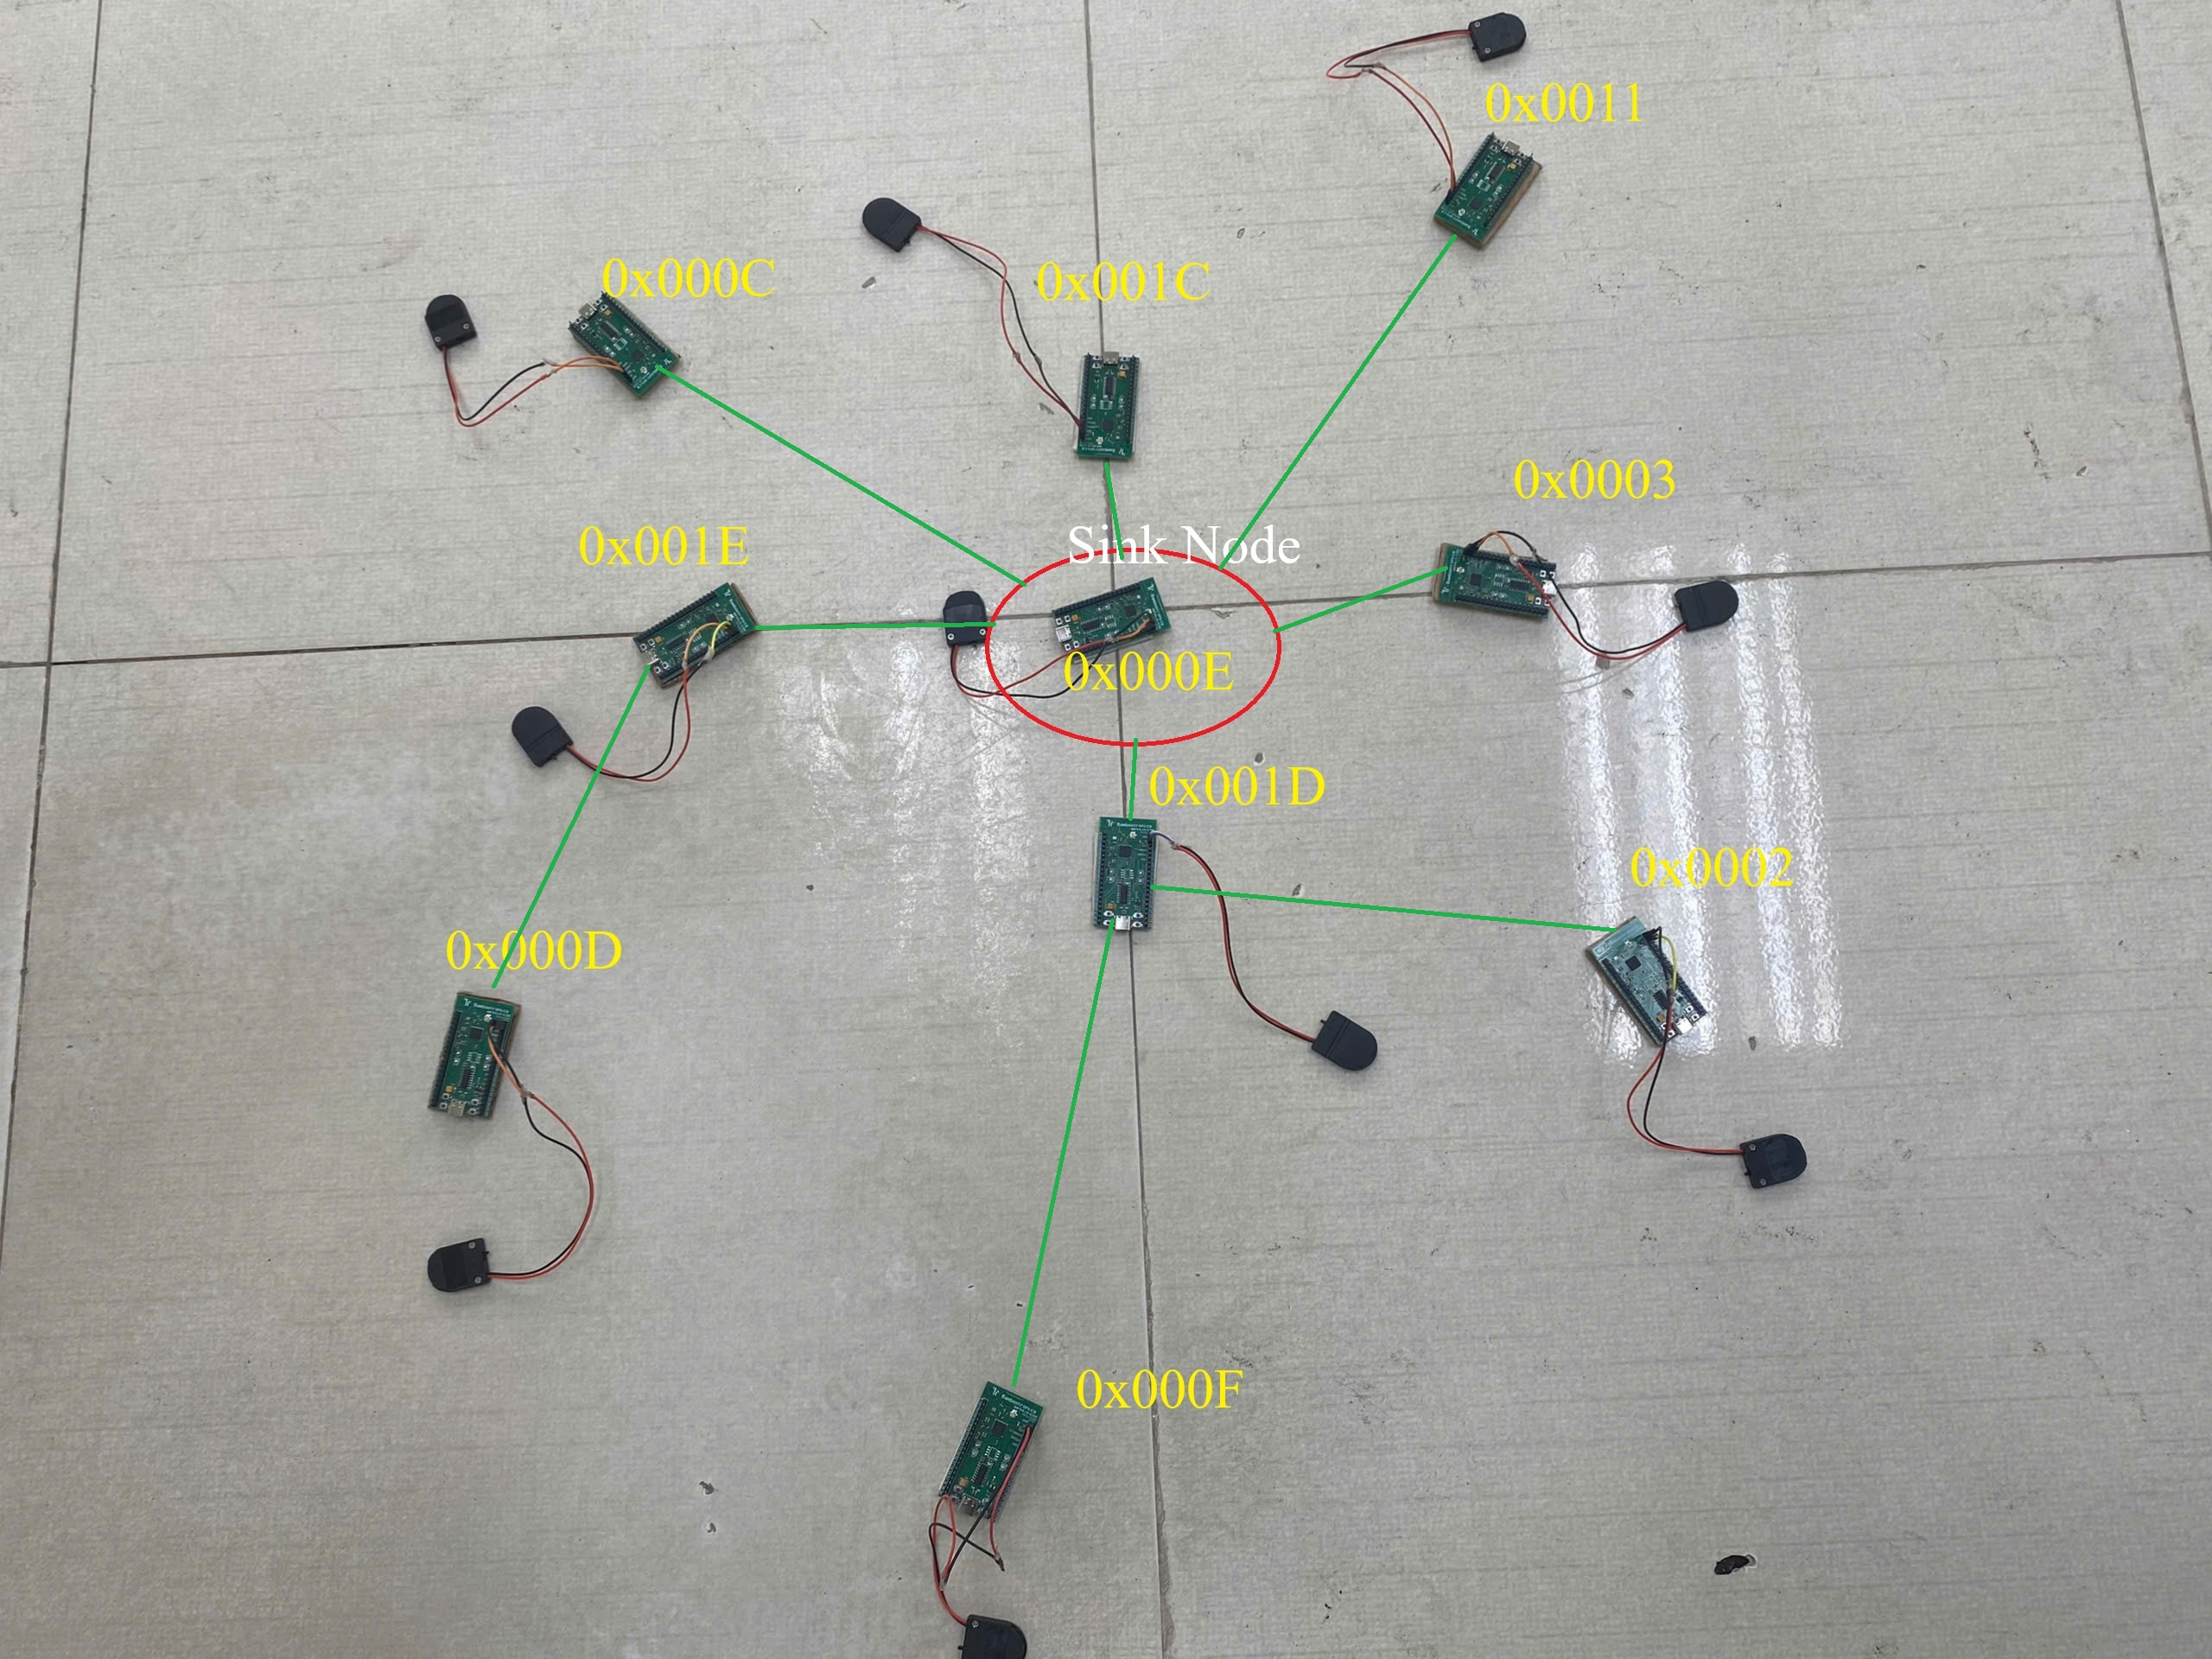
\includegraphics[width=0.60\textwidth]{chapter2/image/demo2.jpg}
    \caption{Topology mạng thí nghiệm dạng lưới}
    \label{fig:grid_topology}
\end{figure}

\clearpage
Tiến hành check log trên từng node trong mạng để kiểm tra bảng định tuyến sau khi quá trình thiết lập gradient hoàn tất. Kết quả hiển thị trong Hình\ref{fig:grid_topology_routing_table}.

\begin{figure}[h!]
    \centering
    
\includegraphics[width=0.75\textwidth]{chapter2/image/demo2/0x000C.png}
    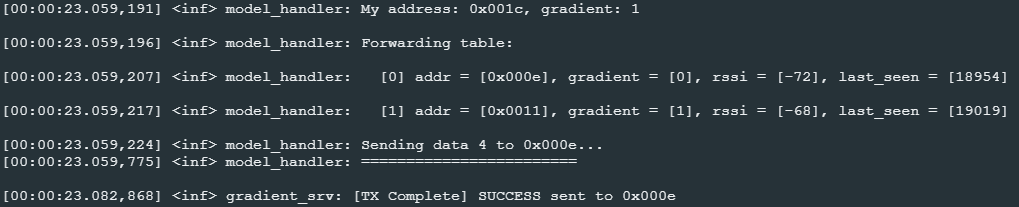
\includegraphics[width=0.75\textwidth]{chapter2/image/demo2/0x001C.png}
    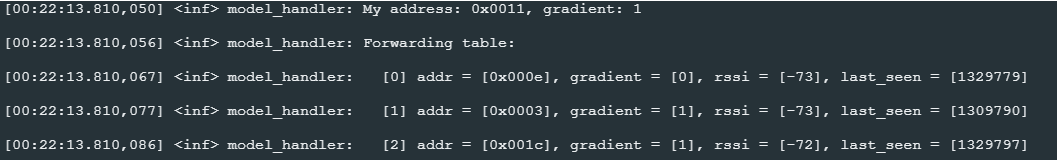
\includegraphics[width=0.75\textwidth]{chapter2/image/demo2/0x0011.png}
    
\includegraphics[width=0.75\textwidth]{chapter2/image/demo2/0x0003.png}
    
\includegraphics[width=0.75\textwidth]{chapter2/image/demo2/0x0002.png}
    
\includegraphics[width=0.75\textwidth]{chapter2/image/demo2/0x001D.png}
    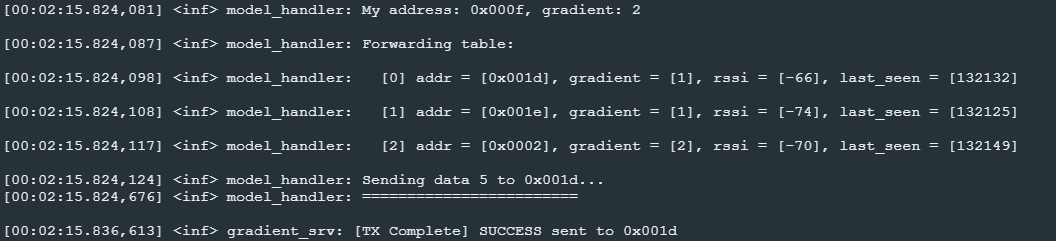
\includegraphics[width=0.75\textwidth]{chapter2/image/demo2/0x000F.png}
    
\includegraphics[width=0.75\textwidth]{chapter2/image/demo2/0x000D.png}
    \caption{Bảng định tuyến tại node các node trong mạng dạng lưới}
    \label{fig:grid_topology_routing_table}
\end{figure}

\subsubsection{Kết quả thí nghiệm}

Quá trình thiết lập gradient trong topology lưới diễn ra tương tự như trong topology cây, các node cập nhật bảng định tuyến và gradient dựa trên các gói tin GRADIENT\_STATUS nhận được từ neighbor đúng như thuật toán đã thiết kế. Tỷ lệ truyền thành công cũng đạt 100\% sau 100 lần truyền gói tin DATA từ các sensor node đến sink node.

\subsection{Nhận xét kết quả thí nghiệm}

Kết quả thí nghiệm cho thấy thuật toán định tuyến Gradient hoạt động hiệu quả trên cả hai loại topology. Topology lưới có ưu thế về độ tin cậy và latency nhờ tính dự phòng cao và vị trí sink tối ưu. Tuy nhiên, topology cây vẫn đạt hiệu suất chấp nhận được và có ưu điểm về độ đơn giản trong triển khai.

Thí nghiệm cũng xác nhận rằng thuật toán thiết lập gradient hội tụ đúng đắn trong cả hai trường hợp, tất cả các node đều cập nhật đúng gradient và bảng định tuyến theo thiết kế. Tỷ lệ truyền thành công 100\% chứng tỏ khả năng chuyển tiếp dữ liệu của thuật toán trong môi trường mạng cấu trúc tĩnh là rất tốt.